\documentclass[10pt]{beamer}
\usepackage{amsmath,amssymb,longtable,hhline}
\usepackage{mathrsfs}
\usepackage{xcolor}
\usepackage{hyperref}
\usepackage{multicol}
\usepackage{anyfontsize}
\usepackage{minted}

\usemintedstyle{tango}
\newcommand{\ltprgsize}{\fontsize{5}{5}\selectfont}
%\newcommand{\ltprgsize}{\footnotesize}
\setminted{fontsize=\footnotesize{},mathescape}

\definecolor{mygreen}{rgb}{0,0.6,0}
\definecolor{mygray}{rgb}{0.5,0.5,0.5}
\definecolor{mymauve}{rgb}{0.58,0,0.82}

\hypersetup{
    bookmarks=true,         % show bookmarks bar?
    unicode=true,           % non-Latin characters in Acrobat’s bookmarks
    pdftoolbar=false,        % show Acrobat’s toolbar?
    pdfmenubar=false,        % show Acrobat’s menu?
    pdffitwindow=false,     % window fit to page when opened
    pdfstartview={FitH},    % fits the width of the page to the window
    pdftitle={Model Driven Architecture Implementation using Linked Data},    % title
    pdfauthor={Evgeny Cherkashin, Alexey Kopaygorodsky, Ljubica Kazi, Alexey Shigarov, Viacheslav Paramonov},     % author
    pdfsubject={model driven architecture},   % subject of the document
    pdfnewwindow=true,      % links in new PDF window
    colorlinks=true,       % false: boxed links; true: colored links
    linkcolor=red,          % color of internal links (change box color with linkbordercolor)
    citecolor=green,        % color of links to bibliography
    filecolor=magenta,      % color of file links
    urlcolor=blue           % color of external links
}

\usepackage{pifont}

\usetheme{Warsaw}
\usecolortheme{crane}
%\useinnertheme{rectangles}
%\setbeamertemplate{itemize item}{\scriptsize\hbox{\donotcoloroutermaths\ding{113}}}
\definecolor{darkding}{RGB}{200,56,0}
\setbeamertemplate{itemize item}{\scriptsize\hbox{\color{darkding}{\bfseries\ding{113}}}}
\setbeamertemplate{itemize subitem}{\tiny\raise1.5pt\hbox{\donotcoloroutermaths$\blacktriangleright$}}
\setbeamertemplate{itemize subsubitem}{\tiny\raise1.5pt\hbox{\donotcoloroutermaths$\blacktriangleright$}}
\setbeamertemplate{enumerate item}{\insertenumlabel.}
\setbeamertemplate{enumerate subitem}{\insertenumlabel.\insertsubenumlabel}
\setbeamertemplate{enumerate subsubitem}{\insertenumlabel.\insertsubenumlabel.\insertsubsubenumlabel}
\setbeamertemplate{enumerate mini template}{\insertenumlabel}

\beamertemplatenavigationsymbolsempty

\usepackage{iftex,ifxetex}
\ifPDFTeX
  \usepackage[utf8]{inputenc}
  \usepackage[T1]{fontenc}
  \usepackage[russian]{babel}
  \usepackage{lmodern}
  \usefonttheme{serif}
\else
  \ifluatex
    \usepackage{unicode-math}
    \defaultfontfeatures{Ligatures=TeX,Numbers=OldStyle}
    \setmathfont{Latin Modern Math}
    \setsansfont{Linux Biolinum O}
    \setmonofont{Fira Mono}[Scale=MatchLowercase]
    \usefonttheme{professionalfonts}
    % \setmathfont[
    %     Ligatures=TeX,
    %     Scale=MatchLowercase,
    %     math-style=upright,
    %     vargreek-shape=unicode
    %     ]{euler.otf}
  \fi
\fi

%\useoutertheme{split}
%\useinnertheme{rounded}
\setbeamertemplate{background canvas}[vertical shading][bottom=white!80!cyan!20,top=cyan!10]
%\setbeamertemplate{sidebar canvas left}[horizontal shading][left=white!40!black,right=black]

\graphicspath{{pics/}}

\providecommand{\email}[1]{\texttt{#1}}

% --------------------------

\begin{document}

\setbeamertemplate{background canvas}[vertical shading][bottom=white,top=white]
\setbeamercolor{background canvas}{bg=white}

\title[Представление Трансформаций MDA в Виде Логических Объектов]{Представление Трансформаций MDA в Виде Логических Объектов} \author[Е. Черкашин, А. Шигаров, В.~Парамонов]{\bfseries \underline{Евгений Черкашин${}^*$}, Алексей Шигаров, Вячеслав Парамонов}
\institute{\normalsize Институт динамики систем и теории управления СО РАН, ул. Лермонтова, д. 134, Иркутск, Россия, 664033\\  [1em] ${}^*$\email{\href{mailto:eugeneai@icc.ru}{eugeneai@icc.ru}} }
\date{Международная конференция\\ Знания-Онтологии-Теории (ЗОНТ 2019)\\ 7--11 Октября, 2019, Новосибирск, Россия}

%%%\date{\today}
\maketitle

\begin{frame} \frametitle{Цели исследования} \textbf{Основная цель} исследования -- создать технологии MDA, которые основаны нв современной системе визуальных языков моделирования (SysML, BPMN, CMMN, и др.), на существующих средствах Семантического Веба: \textbf{форматах}, \textbf{словарях} и \textbf{технологиях}, а также объектно-ориентированном логическом программировании. Следующие технологии и программное обеспечения разрабатываются: \begin{enumerate} \item Представление CIM в виде комплекса моделей SysML, BPMN, CMMN, а также результатов анализа исходного кода, \item Представление CIM, PIM, PSM в формате RDF при помощи известных онтологий, \item реализация трансформации при помощи языка объектного логического программирования Logtalk, \item использование данных серверов LOD для обеспечения дополнительных семантических данных, \item порождение документов и интерфейсов пользователя, размеченных LOD (интеграция ИС в СВ). \end{enumerate} \end{frame} \begin{frame} \frametitle{Технологии-аналоги и стандарты} \begin{itemize} \item Наиболее широко используется язык трансформации ATL и его предшественник QVT -- стандарты OMG; разработаны для преобразования XMI в XMI; \item Использование ATL постепенно восходит на уровень CIM, например, диаграмма BPMN преобразуется в набор диаграмм UML (PIM), используемых для реализации web-приложений, CIM представляется при помощи UML-диаграмм классов и состояний. \item Использование MDA становится шире, например, для анализа аспектов безопасности в распределенных приложениях, при этом результат получается на основе логического вывода над MDA--моделью;
  \item UML используется в качестве CIM/PIM при моделировании онтологий; даже есть специальный стандарт OMG; %\item XML используется для описания сервисов: WSDL, WS-BPEL; %\item MDA is opposed to conceptual programming by Enn Tyugu.
  \end{itemize}

  Трансформация программируется в языке Logtalk, при этом CIM и PIM представляют собой граф RDF, PSM -- это объекты LogTalk. В результате можно использовать не только модели, представленные в стандарте XMI, организовывать многоэтапные трансформации, формируемые из модулей. \end{frame}

\begin{frame} \frametitle{Logtalk как язык задания трансформаций} Язык Logtalk выбран, так как он \begin{itemize} \item наследует синтаксис и среду исполнения программ Prolog; \item реализован как макропакет, при это функционирует всего на 1.5\% медленнее; \item имеет гибкую семантику: можно задавать трансформации и ограничения в рамках одного синтаксиса; \item реализует объектно-ориентированную структуризацию знаний (правил), а также инкапсуляцию и модификацию; \item реализует композицию объектов; \item механизм установки ограничений на сообщения между объектами (события); \item существуют версии для многих реализаций Prolog. \end{itemize} <<Обычные>> языки программирования позволяют использовать библиотеки, которые не имеют прямого отношения к трансформациям MDA.
\end{frame}

\begin{frame}[fragile]
  \frametitle{Использование средств Самантического Веба при представлении исходных моделей}
  \begin{itemize}
  \item Использует опыт исследователей предметных областей, в том числе возведенный в стандарт;
  \item Наборы троек определяют граф (T-Box, A-Box);
  \item Стандартные онтологии заданы формально (\verb|rdfs:domain|, \verb|rdfs:range|);
  \item Поддерживаются практически любыми системами программирования (библиотеки, механизмы вывода/верификации, SPARQL);
  \item В RDF реализован способ глобальной идентификации сущностей, при помощи такого идентификатора можно ссылаться на один и тот же объект из разных систем и моделей;
  \item SWI-Prolog поддерживает прямой доступ к графам RDF, интерпретацию семантики некоторых отношений (\verb|rdfs:label|, \verb|dc:title|); сервер онтологий ClioPatria;
  \item Существует простой способ реализации защиты данных (\verb|rdfs:seeAlso|);
  \item При помощи средств Семантического Веба и принципов LOD можно организовывать интеграцию модулей в гетерогенной информационной среде.
  \end{itemize}
\end{frame}

\begin{frame} \frametitle{Model Driven Architecture и Linked Open Data} \begin{center} 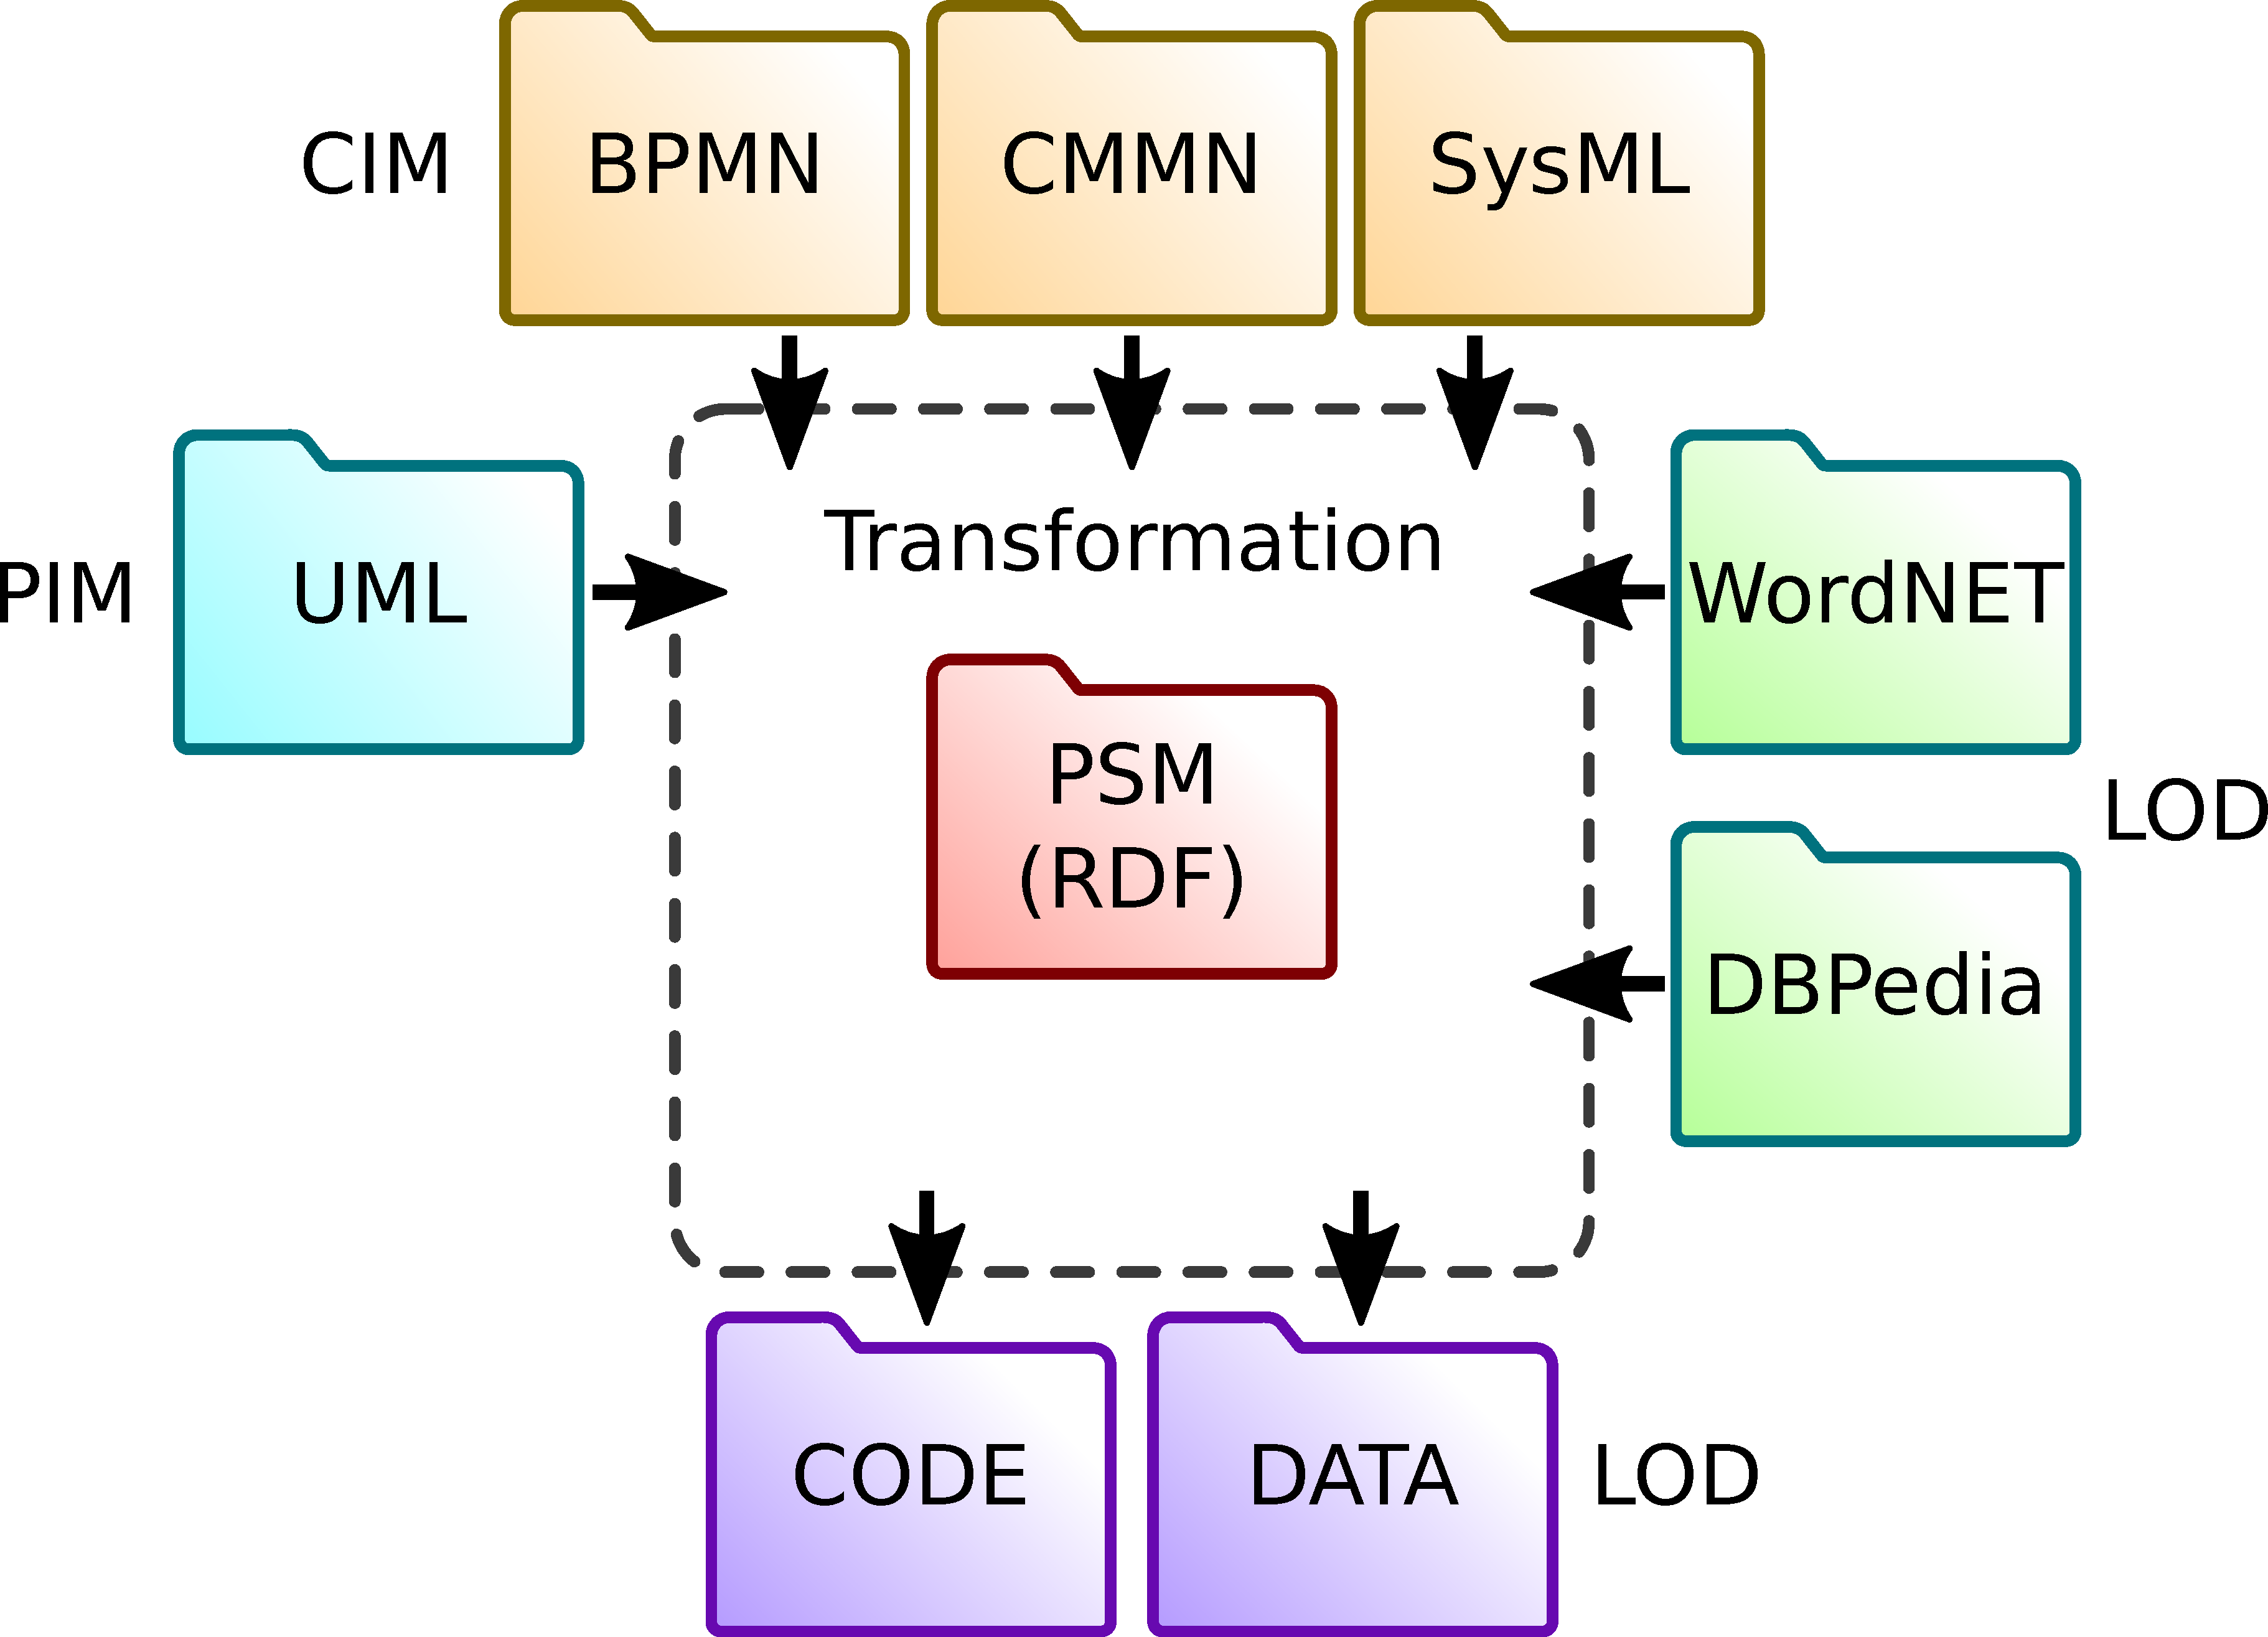
\includegraphics[width=0.9\linewidth]{mda-overview.pdf} \end{center}
\end{frame}


\begin{frame} \frametitle{Инфраструктура MDA} \centering

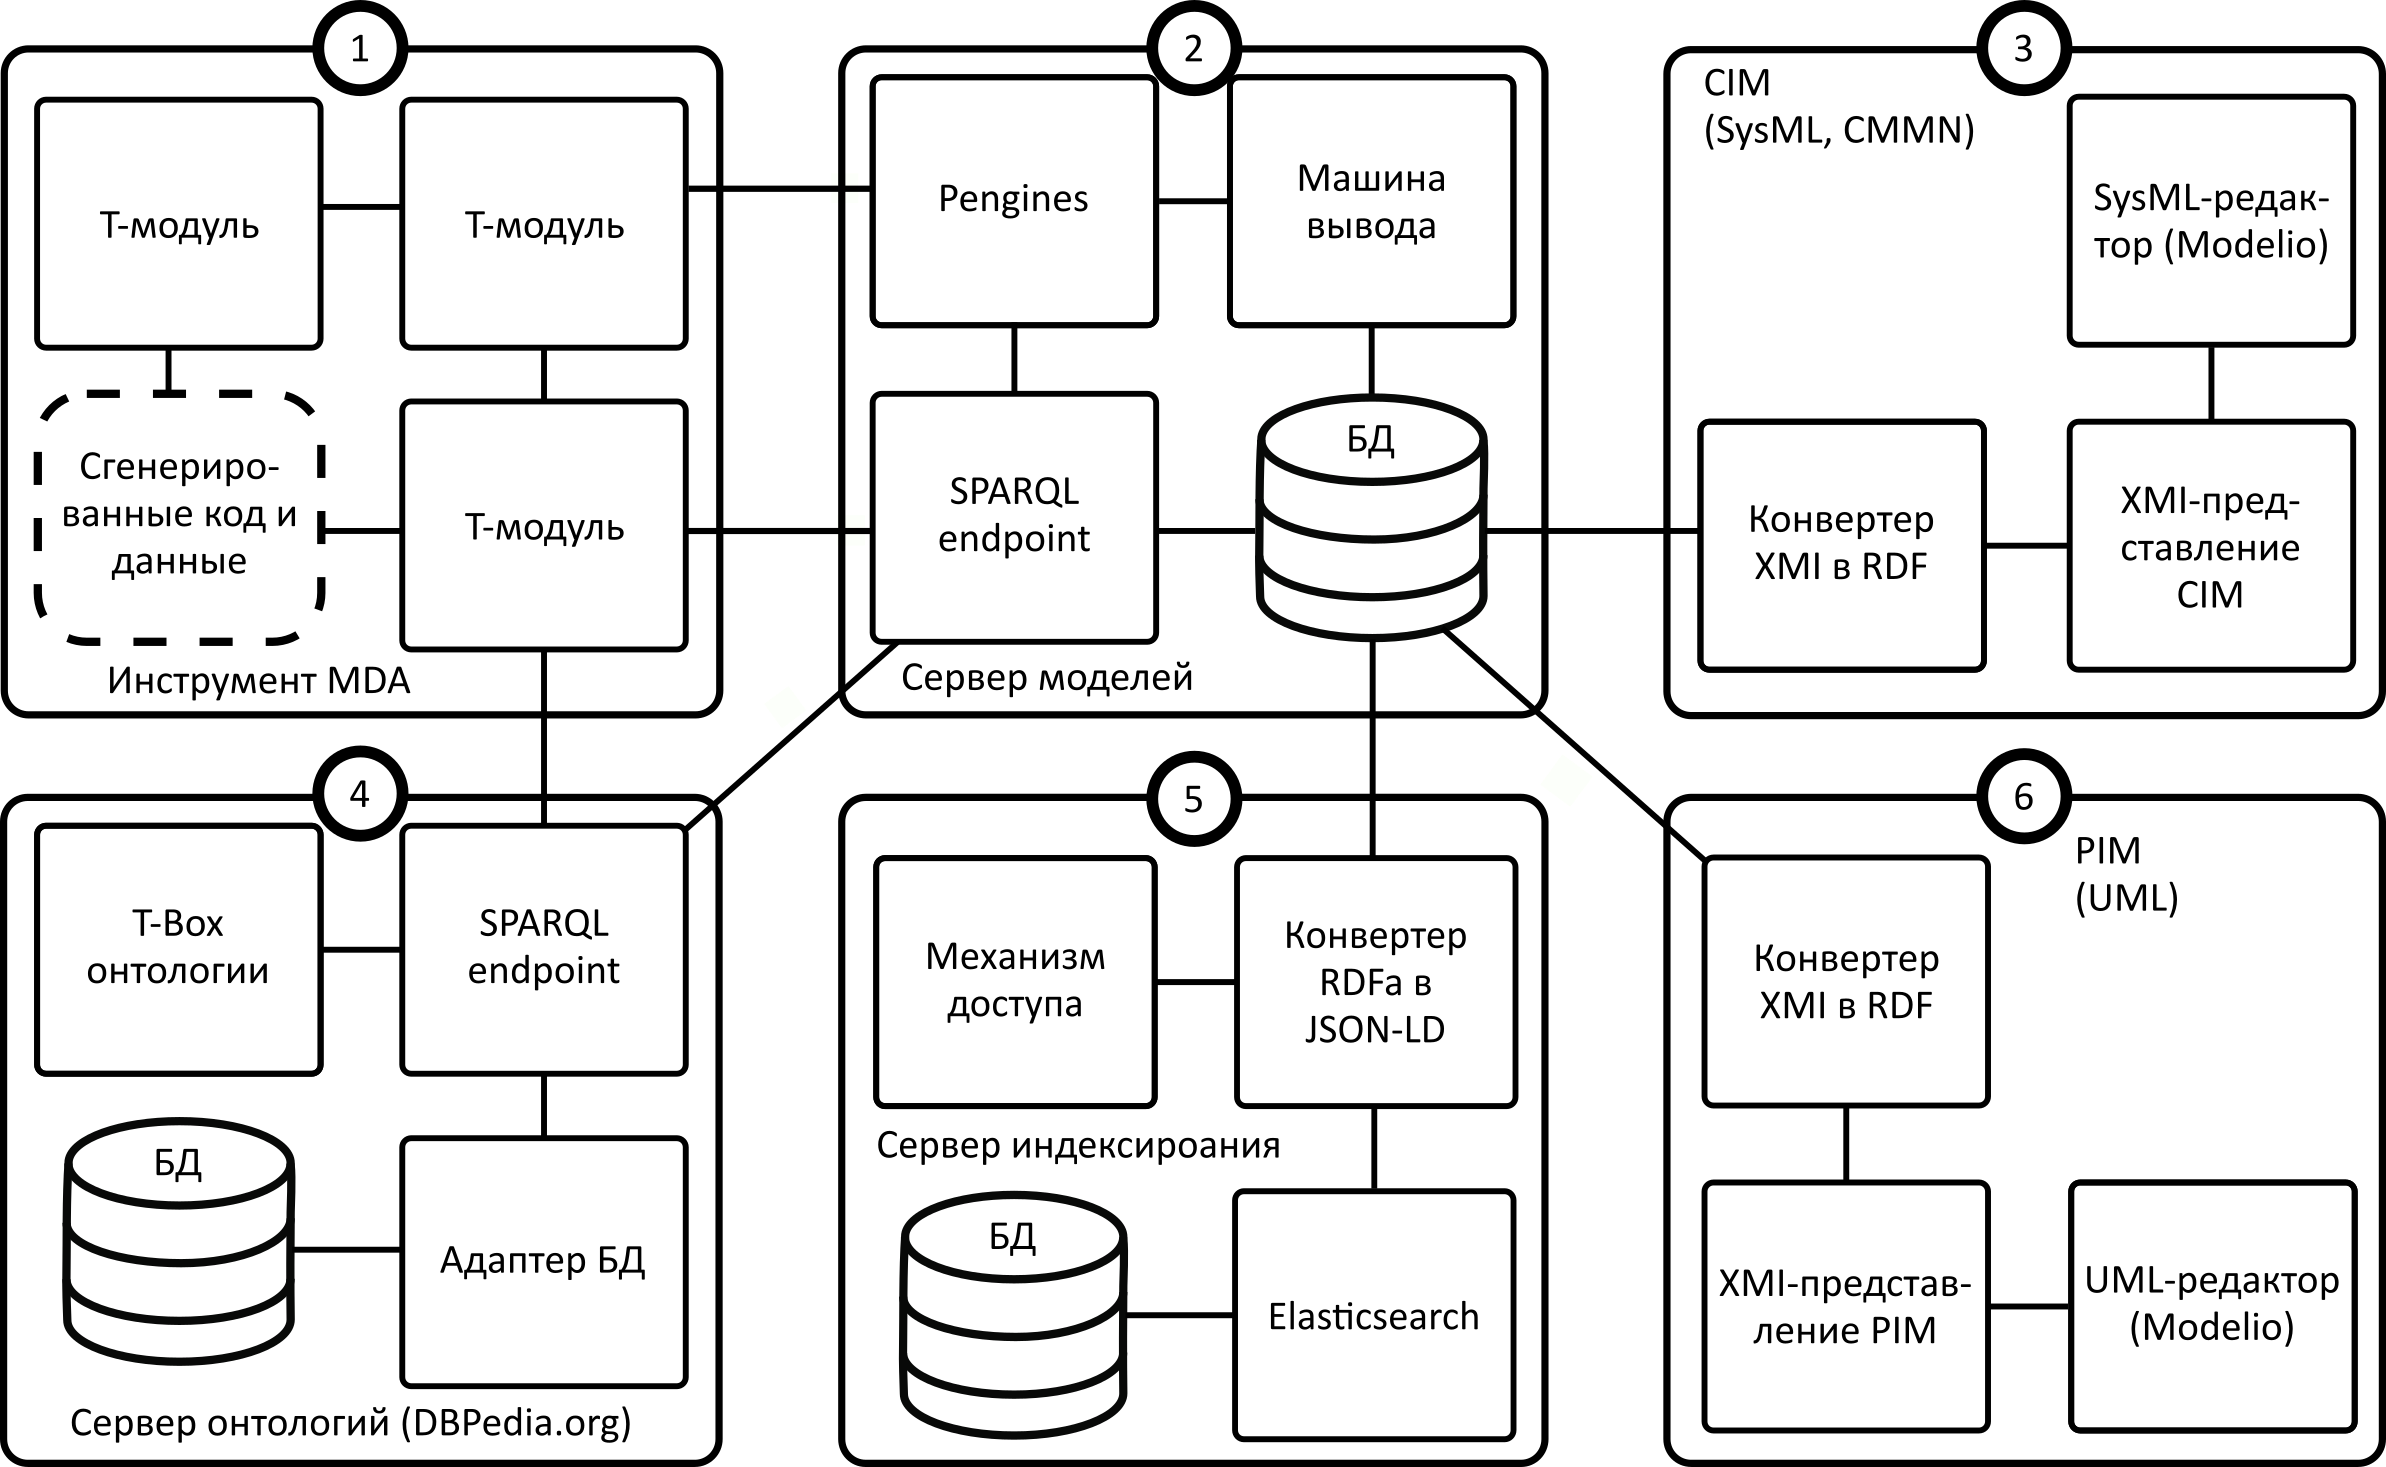
\includegraphics[width=1\linewidth]{architecture-mda-lod-ext-ru.png} \end{frame} \begin{frame} \frametitle{Архитектура модульной системы трансформации} \centering

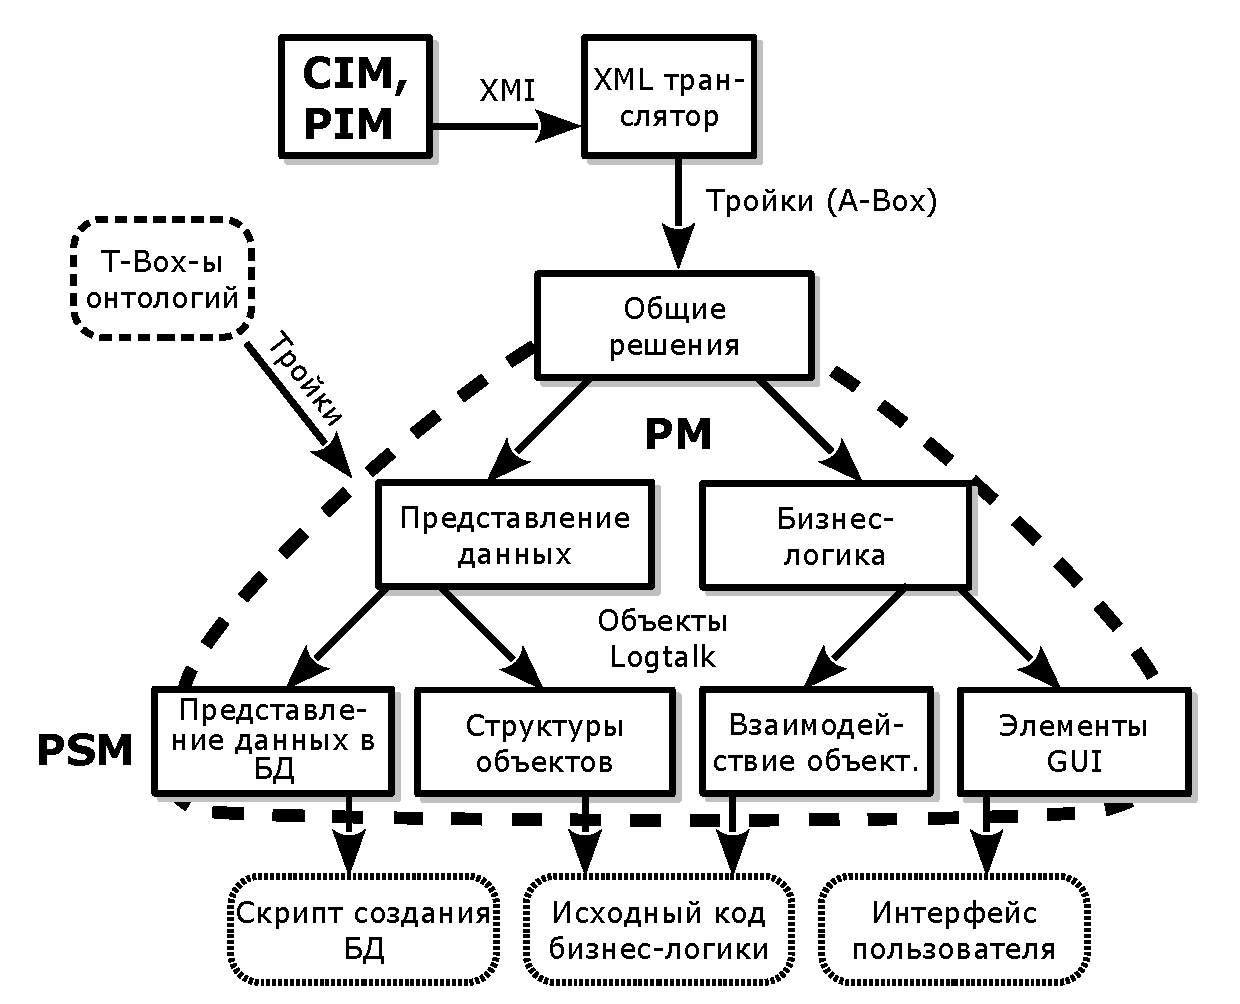
\includegraphics[width=0.9\linewidth]{architect_tree_pres-ru-wo-OCL.pdf} \end{frame}

\begin{frame}[fragile] \frametitle{PSM: Сценарий синтеза класса}


%\begin{multicols}{2}
  \begin{columns}
    \begin{column}{0.6\textwidth}
\begin{minted}[fontsize=\tiny]{logtalk}
:- object(direct(_Package,_LocalProf,_CodeProf)).    % Transformation driver object
:- public([tr/4,tr/3]).                              % Public interface of a class synthesis scenario
% . . . . . . . . . .
tr(class, Class, ClassID):- ::package(Package),      % Synthesize a class
    query(Package)::class(Name, ClassID),            % Query package structure in XMI
    create_object(Class,      % . . . . .            % Create a <<Class>> object
    create_object(Attributes, % . . . . .            % Create <<Attributes>> object
    create_object(Methods,    % . . . . .            % ...<<Methods>>.
    Class::name(Name),                               % Name the class.
    % Generate attributes of the class,
    % organizing them in a local database.
    % ...methods...
    Class::attributes(Attributes),                   % Set the attributes for class.
    Class::methods(Methods).                         % ...methods.

tr(attribute, Attribute, ClassID, AttributeID):-     % Attribute transformations
    ::package(Package),
    query(Package)::attribute(Name,ClassID,AttrID),
    create_object(Attribute,  % . . . . .
    Attribute::name(Name).                           % Name the attribute.

tr(method, Method, ClassID, MethodID):-              % Transformation of methods
    ::package(Package),
    query(Package)::method(Name,ClassID,MethodID),
    create_object(Method,     % . . . . .
    Method::name(Name).                              % Name of the method
:- end_object.
\end{minted}
    \end{column}
    \begin{column}{0.4\linewidth}
      
\includegraphics[width=1\linewidth]{scenario-ru.png}
    \end{column}
  \end{columns}
  % \end{multicols}
\end{frame}

\begin{frame}[fragile]
  \frametitle{Реализация объекта \texttt{Query}} \begin{minted}[fontsize=\footnotesize{}]{logtalk}
:- object(query(_XMI)).
:- protected(xmi/1).
:- public([class/2, attribute/3, method/3]).
xmi(XMI) :- parameter(1, XMI).
class(Name, ID):-                            % Recognition of Class in RDF
    ::xmi(XMI),
    XMI::rdf(ID,rdf:type,uml:'Class'),
    XMI::rdf(ID,rdfs:label, literal(Name)).
attribute(Name, ClassID, ID):-               % ...attribute...
    ::xmi(XMI),
    XMI::rdf(ClassID, xmi:ownedAttribute, ID),
    XMI::rdf(ID, rdfs:label, literal(Name)).
method(Name, ClassID, ID):-                  % ...method...
    ::xmi(XMI),
    XMI::rdf(ClassID, xmi:ownedOperation, ID),
    XMI::rdf(ID, rdfs:label, literal(Name)).
% . . . . . . . . . . .
:- end_object.
\end{minted}
\end{frame}

\begin{frame}[fragile] \frametitle{Класс Code Block (идея взята в \texttt{llvmlite}${}^*$)}
  \begin{columns}
    \begin{column}{0.6\textwidth}
      \flushleft
\begin{minted}[fontsize=\footnotesize{}]{logtalk}
:- object(code_block, specializes(root)).
% Public interface of the object
:- public([append/1, prepend/1, clear/0,
   render/1, render_to/1, remove/1,
   item/1, items/1]).
% Code block items
:- dynamic([item_/1]).
:- private([item_/1]).
% Methods specialized during inheritance
:- protected([renderitem/2, render_to/2]).
% . . . . . . . . . . . .
% Delegate rendering to object itself
renderitem(Object, String):-
    current_object(Object), !,
    Object::render(String).
% Convert a literal to its string
% representation
renderitem(literal(Item), String):-!,
    atom_string(Item, String).
% Just print the item (debugging).
renderitem(Item, String):-
    root::iswritef(String, '%q', [Item]).
:- end_object.
\end{minted}
    \end{column}
    \begin{column}{0.4\textwidth}
      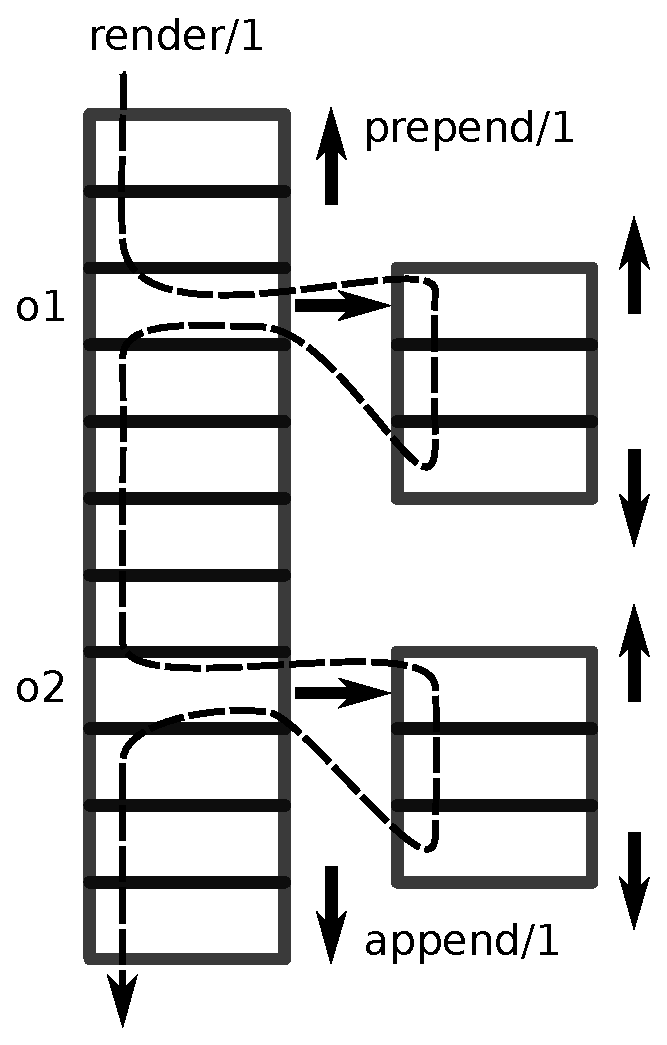
\includegraphics[width=1\linewidth]{code_block.pdf}
  ${}^*$) \url{https://github.com/numba/llvmlite}
    \end{column}
  \end{columns}
 \end{frame}

\begin{frame}[fragile] \frametitle{PSM класса Python, специализации Code Block}

\begin{columns} \begin{column}{0.6\textwidth} \flushleft

\begin{minted}[fontsize=\scriptsize]{logtalk}
:- object(class, specializes(code_block),
   imports([named])). % Category of named entities
:- public([classlist/1, methods/1, attributes/1]).
% . . . . . . . . . . . . . .
renderitem(Item, Result):-      % proceed with default
    ^^renderitem(Item, Result). % rendering
render(Result):-         % Source generator
    ^^render(Name),      % implemented in a category
    ( ::item(classlist(List)) ->
     % . . . . . . . . . . .
        [Name]) ),
    ( ::item(attributes(Attributes))->
     % . . . . . . . . . . .
        [DefAttrList]),
      Attributes::items(InstanceAttrs),
      findall(S, ( % initialize attributes
         % . . . . . . . . .
         ), AttrAssigns),
        root::unindent,
        AttrList=[ConstructorDef|AttrAssigns];
         % . . . . . . . . .
        AttrList=[ConstructorDef, Pass] ),
    ( ::item(methods(Methods))-> % If any ...
      Methods::render(MethodList);
      MethodList=[] ),
    lists::append(AttrList,MethodList,StringList),
    root::unindent, Result=[Signature|StringList].
:- end_object.
\end{minted}
\end{column} \begin{column}{0.4\linewidth} 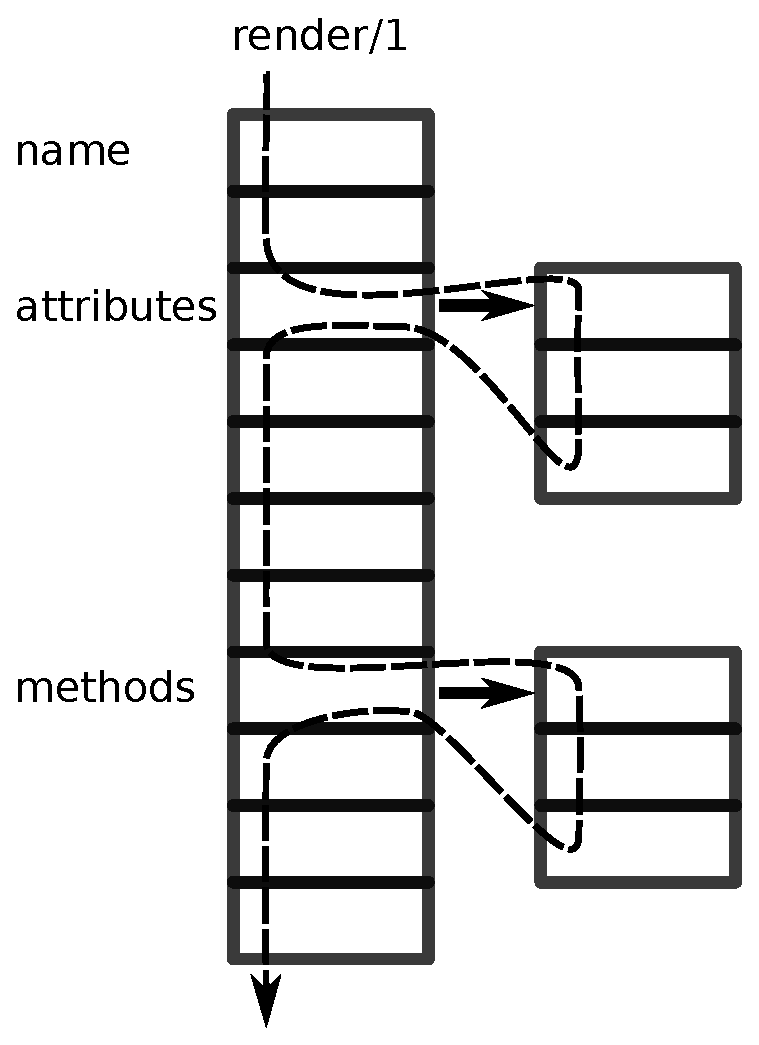
\includegraphics[width=1\linewidth]{code_block_class.pdf} \end{column} \end{columns}

% If any ...% \end{multicols}
\end{frame}

\begin{frame}[fragile] \frametitle{Категории Logtalk} Категория поименованных сущностей
\begin{minted}[fontsize=\scriptsize]{logtalk}
:- category(named).
:- public([name/1, render/1]).
:- protected([renderitem/2]).
name(Name):- ::prepend(name(Name)).
renderitem(name(Name), String):-!, atom_string(Name, String).
render(String):-  % What is code generation from items
    ::item(name(Name)), ::renderitem(name(Name), String).
:-end_category.
\end{minted}

Категория поименованных сущностей некоторого типа
\begin{minted}[fontsize=\scriptsize]{logtalk}
:- category(namedtyped, extends(named)).
:- public([type/1,render/2, separator_option/2,list_separator/1]).
:- protected([renderitem/2]).
type(Type):- ::append(type(Type)).
renderitem(Item, String):- ^^renderitem(Item, String),!.
renderitem(type(Type),String):-!, ::list_separator(Separator),
    writef::swritef(String, '%w%w', [Separator, Type]).
render(Middle, String):- ^^render(SName),
    (   ::item(type(Type)) ->
        ::renderitem(type(Type), SType),
        string_concat(SName, Middle, _1),
        string_concat(_1, SType, String) ;
        SName = String  ).
render(String):-  ::render("", String).
list_separator(Separator):-
    ::separator_option(Name, Default),!, % Global options
    root::option(Name, Separator, Default).
:- end_category.

\end{minted}
\end{frame}

\begin{frame}[fragile] \frametitle{Доступ к данным LOD}


  \begin{columns}
\begin{column}{0.5\textwidth}
\begin{minted}[fontsize=\scriptsize]{logtalk}
:- category(sparql).
:- public(query/2).
query(Pattern,Parameters,Row):-
    prepare(Pattern,Parameters,Query),
    server(Host,Port,Path),
    sparql_query(Query, Row,
        [host(Host),port(Port),path(Path)]).
:- protected(server/3).  % must be implemented
                         % by a subclass.
:- protected(prepare/3). % prepares a query
% . . . . . . . . . .    %             string.
:- end_category.

:- object(dbpedia, imports(sparql)).
:- protected(server/3).
server('dbpedia.org',80,'/sparql').
:- public(entity_name/2).
entity_name(Entity,Language,Name):-
    query('select ?name where { '
          ' %w rdfs:label ?name. '
          'FILTER langMatches( lang(?label),'
          ' "%w" )}', [Entity, Language],
          row(Name)).
:- end_object.

% ?- dbpedia::entity_name(dbr:'Passport', 'ru', Name).
\end{minted}
\end{column}
\begin{column}{0.5\textwidth}
  \flushright
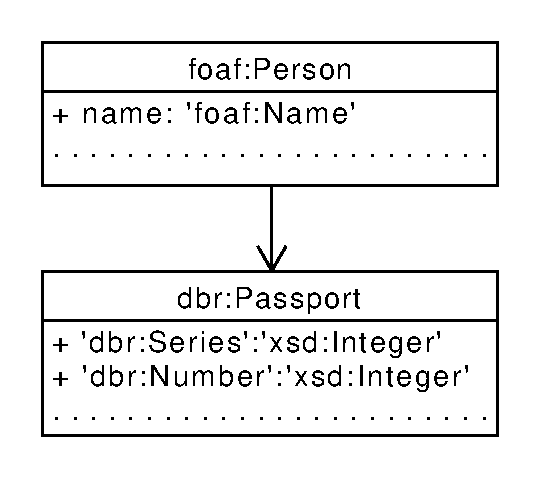
\includegraphics[width=0.8\linewidth]{simple-diag.pdf}
\end{column}
\end{columns}
 \end{frame}

\begin{frame} \frametitle{Приложение: Представление анализа ампликонов в NGS в виде dataflow-диаграмм} \begin{columns} \begin{column}{0.6\textwidth} \begin{raggedright} 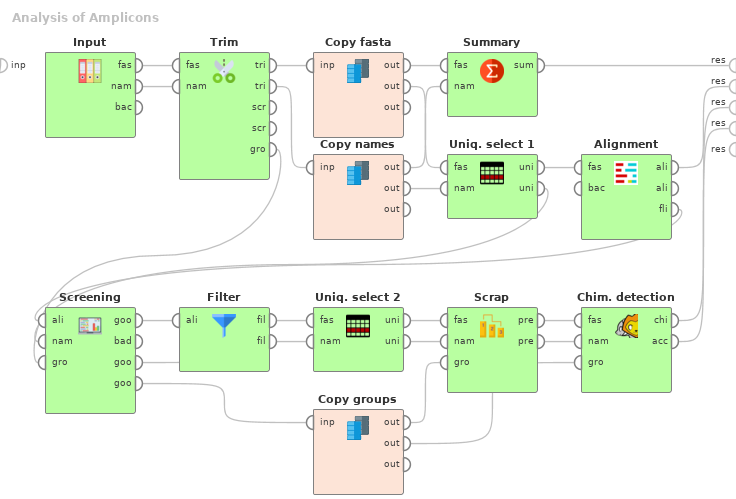
\includegraphics[width=1\linewidth]{Dataflow-color-en.png} \end{raggedright} \end{column} \begin{column}{0.4\textwidth}\footnotesize \begin{tabular}{ll} Term &Расшифровка\\ \hline

NGS &New Generation\\ &Sequencing\\ Amplicon &Часть ДНК или РНК,\\ &скопированная много раз\\ Mothur &Прикладной пакет для\\ &исследований в NGS\\ Rapidminer &Инструмент визуального моделирования \\ &процедур анализа данных\\ &и их исполнения \end{tabular} ${}$\\[1em] Зеленые блоки -- модули Mothur. Остальные -- модули Rapidminer. \end{column} \end{columns} \end{frame}

\begin{frame} \frametitle{Дискуссия} Получен интересный позитивный опыт: \begin{itemize} \item Logtalk и RDF очень гибки, универсальны, и удобны при реализации трансформаций в MDA; \item Наиболее полезный приемы программирования -- это инкапсуляция "сложного" в предикаты--методы и инкапсуляция наборов правил в объекты Logtalk; \item Не все инструменты и приемы программирования Logtalk освоены: необходимо их изучить и выработать методики их использования, например, для инструментов перехвата сообщений (watchers). \end{itemize} Некоторые технические проблемы немного портят общий оптимизм: \begin{itemize} \item Очень простые задачи при использовании MDA требуют несоизмеримых усилий, например, обработка текстов: преобразование идентификатора в CamelCase; \item Много времени занимает поиск подходящей онтологии в интернете, но это все же продуктивнее, чем собственная разработка; \item Prolog не самый популярный язык программирования в MDA, то же и для LogTalk. \end{itemize} \end{frame}

\begin{frame} \frametitle{Заключение} К настоящему времени получены следующие результаты: \begin{itemize} \item Методика представления моделей разработана и в некоторой степени протестирована. \item Создана методика объектно-ориентированного программирования процедур трансформации для языка Logtalk. \item Реализованы прототипы для некоторых трансформаций. \item Средства трансформаций апробированы в прикладной области, сложных проблем пока не выявлено. \end{itemize} Дальнейшее развитие видим по следующим направлениям: \begin{itemize} \item Разработка методики автоматизации разметки отчетных документов LOD. \item Развитие методики реализаций модулей трансформаций с минимальным использованием динамических объектов, используя свойства Logtalk как макропакета. \item Сформировать современный инструментарий разработки ИС из существующего прототипа. \end{itemize}
 Исходный код хранится на сервере \url{https://github.com/isu-enterprise/icc.xmitransform}, \url{https://github.com/eugeneai/icc.mothurpim}.
\end{frame}

\begin{frame} \begin{center} \Large Спасибо за проявленный интерес к нашему проекту! \end{center} \end{frame}

\begin{frame}[fragile]
  \frametitle{Исходный код модуля NGS в Rapidminer}
\begin{minted}[fontsize=\tiny]{cpp}
vector<string> AlignCommand::setParameters(){ // PART OF MODULE SOURCE
try {
  CommandParameter ptemplate("reference", "InputTypes", "", "", "none", "none", "none","",false,true,true); parameters.push_back(ptemplate);
  CommandParameter pcandidate("fasta", "InputTypes", "", "", "none", "none", "none","fasta-alignreport-accnos",false,true,true); parameters.push_back(pcandidate);
  CommandParameter psearch("search", "Multiple", "kmer-blast-suffix", "kmer", "", "", "","",false,false,true); parameters.push_back(psearch);
  CommandParameter pksize("ksize", "Number", "", "8", "", "", "","",false,false); parameters.push_back(pksize);
  CommandParameter pmatch("match", "Number", "", "1.0", "", "", "","",false,false); parameters.push_back(pmatch);
// . . . . . . .
\end{minted}
\begin{minted}[fontsize=\tiny]{java}
package com.rapidminer.ngs.operator; // GENERATED JAVA MODULE
// imports

class MothurChimeraCcodeOperator extends MothurGeneratedOperator {
  private InputPort fastaInPort = getInputPorts().createPort("fasta");
  private InputPort referenceInPort = getInputPorts().createPort("reference");
  private OutputPort chimeraOutPort = getOutputPorts().createPort("chimera");
  private OutputPort mapinfoOutPort = getOutputPorts().createPort("mapinfo");
  private OutputPort accnosOutPort = getOutputPorts().createPort("accnos");

  public MothurChimeraCcodeOperator (OperatorDescription description) {
    super(description);
  }
  @Override
  public void doWork() throws OperatorException {
    super();
    // . . . . . .
  }
  @Override
  public List<ParameterType> getParameterTypes() {
    super();
        // . . . . . .
  }
  @Override
  public String getOutputPattern(String type) {
    if (type=="chimera") return "[filename],[tag],ccode.chimeras-[filename],ccode.chimeras";
    if (type=="mapinfo") return "[filename],mapinfo";
    if (type=="accnos") return "[filename],[tag],ccode.accnos-[filename],ccode.accnos";
    return super.getOutputPattern(type);
  }
}
\end{minted}
\end{frame}

\begin{frame}[fragile]
  \frametitle{Представление исходного кода Mothur в RDF (TTL) и его объект-фасад query}
\begin{multicols}{2}
\begin{minted}[fontsize=\tiny]{turtle}
@prefix xml: <http://www.w3.org/XML/1998/namespace> .
@prefix xsd: <http://www.w3.org/2001/XMLSchema#> .
ngsp:spec a ngsp:Specification ;
    ngsp:module mothur:NoCommand,
        mothur:align-check,
        mothur:align-seqs,
# . . . . .
mothur:align-check a ngsp:Module ;
    ngsp:outputPattern [ a cnt:Chars ;
            ngsp:parameterName "type" ;
            ngsp:pattern [ ngsp:patternString
                    "[filename],align.check" ;
                    dc:identifier "aligncheck" ] ;
            cnt:chars # . . . .
# . . . . .
mothur:align-check-idir-parameter a ngsp:Parameter ;
    ngsp:important false ;
    ngsp:multipleSelectionAllowed false ;
    ngsp:optionsDefault "" ;
    ngsp:required false ;
    ngsp:type mothur:String ;
    dc:title "inputdir" .

mothur:align-check-map-parameter a ngsp:Parameter ;
    ngsp:important true ;
    ngsp:multipleSelectionAllowed false ;
    ngsp:optionsDefault "" ;
    ngsp:required true ;
    ngsp:type mothur:InputTypes ;
    dc:title "map" .

mothur:align-check-name-parameter a ngsp:Parameter ;
    ngsp:chooseOnlyOneGroup "namecount" ;
    ngsp:important false ;
    ngsp:multipleSelectionAllowed false ;
# . . . . .
\end{minted}
\begin{minted}[fontsize=\tiny]{logtalk}
:- object(queryparam(_RDF,_Parameter),
          extends(ngsquerybase)).

:- public(type/1).
type(Type) :-
    ::attr(type, Type).
:- public(name/1).
name(Name) :- ::attr(dc:title, literal(Name)).
:- public(options/1).
options(Value):- ::attr(options, Value).
:- public(options_default/1).
options_default(Value):-
    ::attr(optionsDefault, Value).
% . . . . . . . .
:- public(multiple_selection_allowed/0).
multiple_selection_allowed:-
    ::bool_attr(multipleSelectionAllowed).
:- public(required/0).
required:-
    ::bool_attr(required).
:- public(important/0).
important:-
    ::bool_attr(important).
:- protected(attr/2).
attr(NS:Name, Value):-
    ::ngs(RDF),
    ::second(Parameter),
    rdf_db::rdf_global_object(Value, V),
    RDF::rdf(Parameter, NS:Name, V).
attr(Name, Value):-
    \+ Name=_:_,!,
    ::ngs(RDF),
    ::second(Parameter),
    rdf_db::rdf_global_id(Value, V),
    RDF::rdf(Parameter, ngsp:Name, V).
% . . . . .
:- end_object.

\end{minted}
\end{multicols}
\end{frame}

\end{document}

%%% Local Variables:
%%% mode: latex
%%% TeX-master: t
%%% End:
